\documentclass[]{article}

% Imported Packages
%------------------------------------------------------------------------------
\usepackage{amssymb}
\usepackage{amstext}
\usepackage{amsthm}
\usepackage{amsmath}
\usepackage{enumerate}
\usepackage{fancyhdr}
\usepackage[margin=1in]{geometry}
\usepackage{graphicx}
\usepackage{extarrows}
\usepackage{setspace}
%------------------------------------------------------------------------------

% Header and Footer
%------------------------------------------------------------------------------
\pagestyle{plain}
\renewcommand\headrulewidth{0.4pt}
\renewcommand\footrulewidth{0.4pt}
%------------------------------------------------------------------------------

% Title Details
%------------------------------------------------------------------------------
\title{Deliverable \#1 Template}
\author{SE 3A04: Software Design II -- Large System Design}
\date{}
%------------------------------------------------------------------------------

% Document
%------------------------------------------------------------------------------
\begin{document}

\maketitle

\section{Introduction}
\label{sec:introduction}
% Begin Section

This section of the SRS should provide an overview of the entire SRS.

\subsection{Purpose}
\label{sub:purpose}
% Begin SubSection
\begin{enumerate}[a)]
	\item Delineate the purpose of the SRS
	\item Specify the intended audience for the SRS
\end{enumerate}
% End SubSection

\subsection{Scope}
\label{sub:scope}
% Begin SubSection
\begin{enumerate}[a)]
	\item Identify the software product(s) to be produced by name (e.g., Host DBMS, Report Generator, etc.)
	\item Explain what the software product(s) will, and, if necessary, will not do
	\item Describe the application of the software being specified, including relevant benefits, objectives, and goals
	\item Be consistent with similar statements in higher-level specifications (e.g., the system requirements specification), if they exist
\end{enumerate}
% End SubSection

\subsection{Definitions, Acronyms, and Abbreviations}
\label{sub:definitions_acronyms_and_abbreviations}
% Begin SubSection
\begin{enumerate}[a)]
	\item Provide the definitions of all terms, acronyms, and abbreviations required to properly interpret the SRS
\end{enumerate}
% End SubSection

\subsection{References}
\label{sub:references}
% Begin SubSection
\begin{enumerate}[a)]
	\item Provide a complete list of all documents referenced elsewhere in the SRS
	\item Identify each document by title, report number (if applicable), date, and publishing organization
	\item Specify the sources from which the references can be obtained
\end{enumerate}
% End SubSection

\subsection{Overview}
\label{sub:overview}
% Begin SubSection
\begin{enumerate}[a)]
	\item Describe what the rest of the SRS contains
	\item Explain how the SRS is organized
\end{enumerate}
% End SubSection

% End Section

\section{Overall Description}
\label{sec:overall_description}
% Begin Section

This section of the SRS should describe the general factors that affect the product and its requirements. It does not state specific requirements; it provides a background for those requirements and makes them easier to understand.

\subsection{Product Perspective}
\label{sub:product_perspective}
% Begin SubSection
Plan 6 is a distributed learning management system designed to facilitate teachers and students with everyday classroom operations. Plan 6 is a distributed, self-contained system with several components running on different end-user devices. Plan 6 is akin to other learning management systems, such as McMaster's Avenue2Learn; however, Plan 6 will focus on providing a Learning Management System for early learners and educators with low levels of technical expertise. 

A block diagram denoting the major components of system as well as their external interfaces follow:

\begin{center}
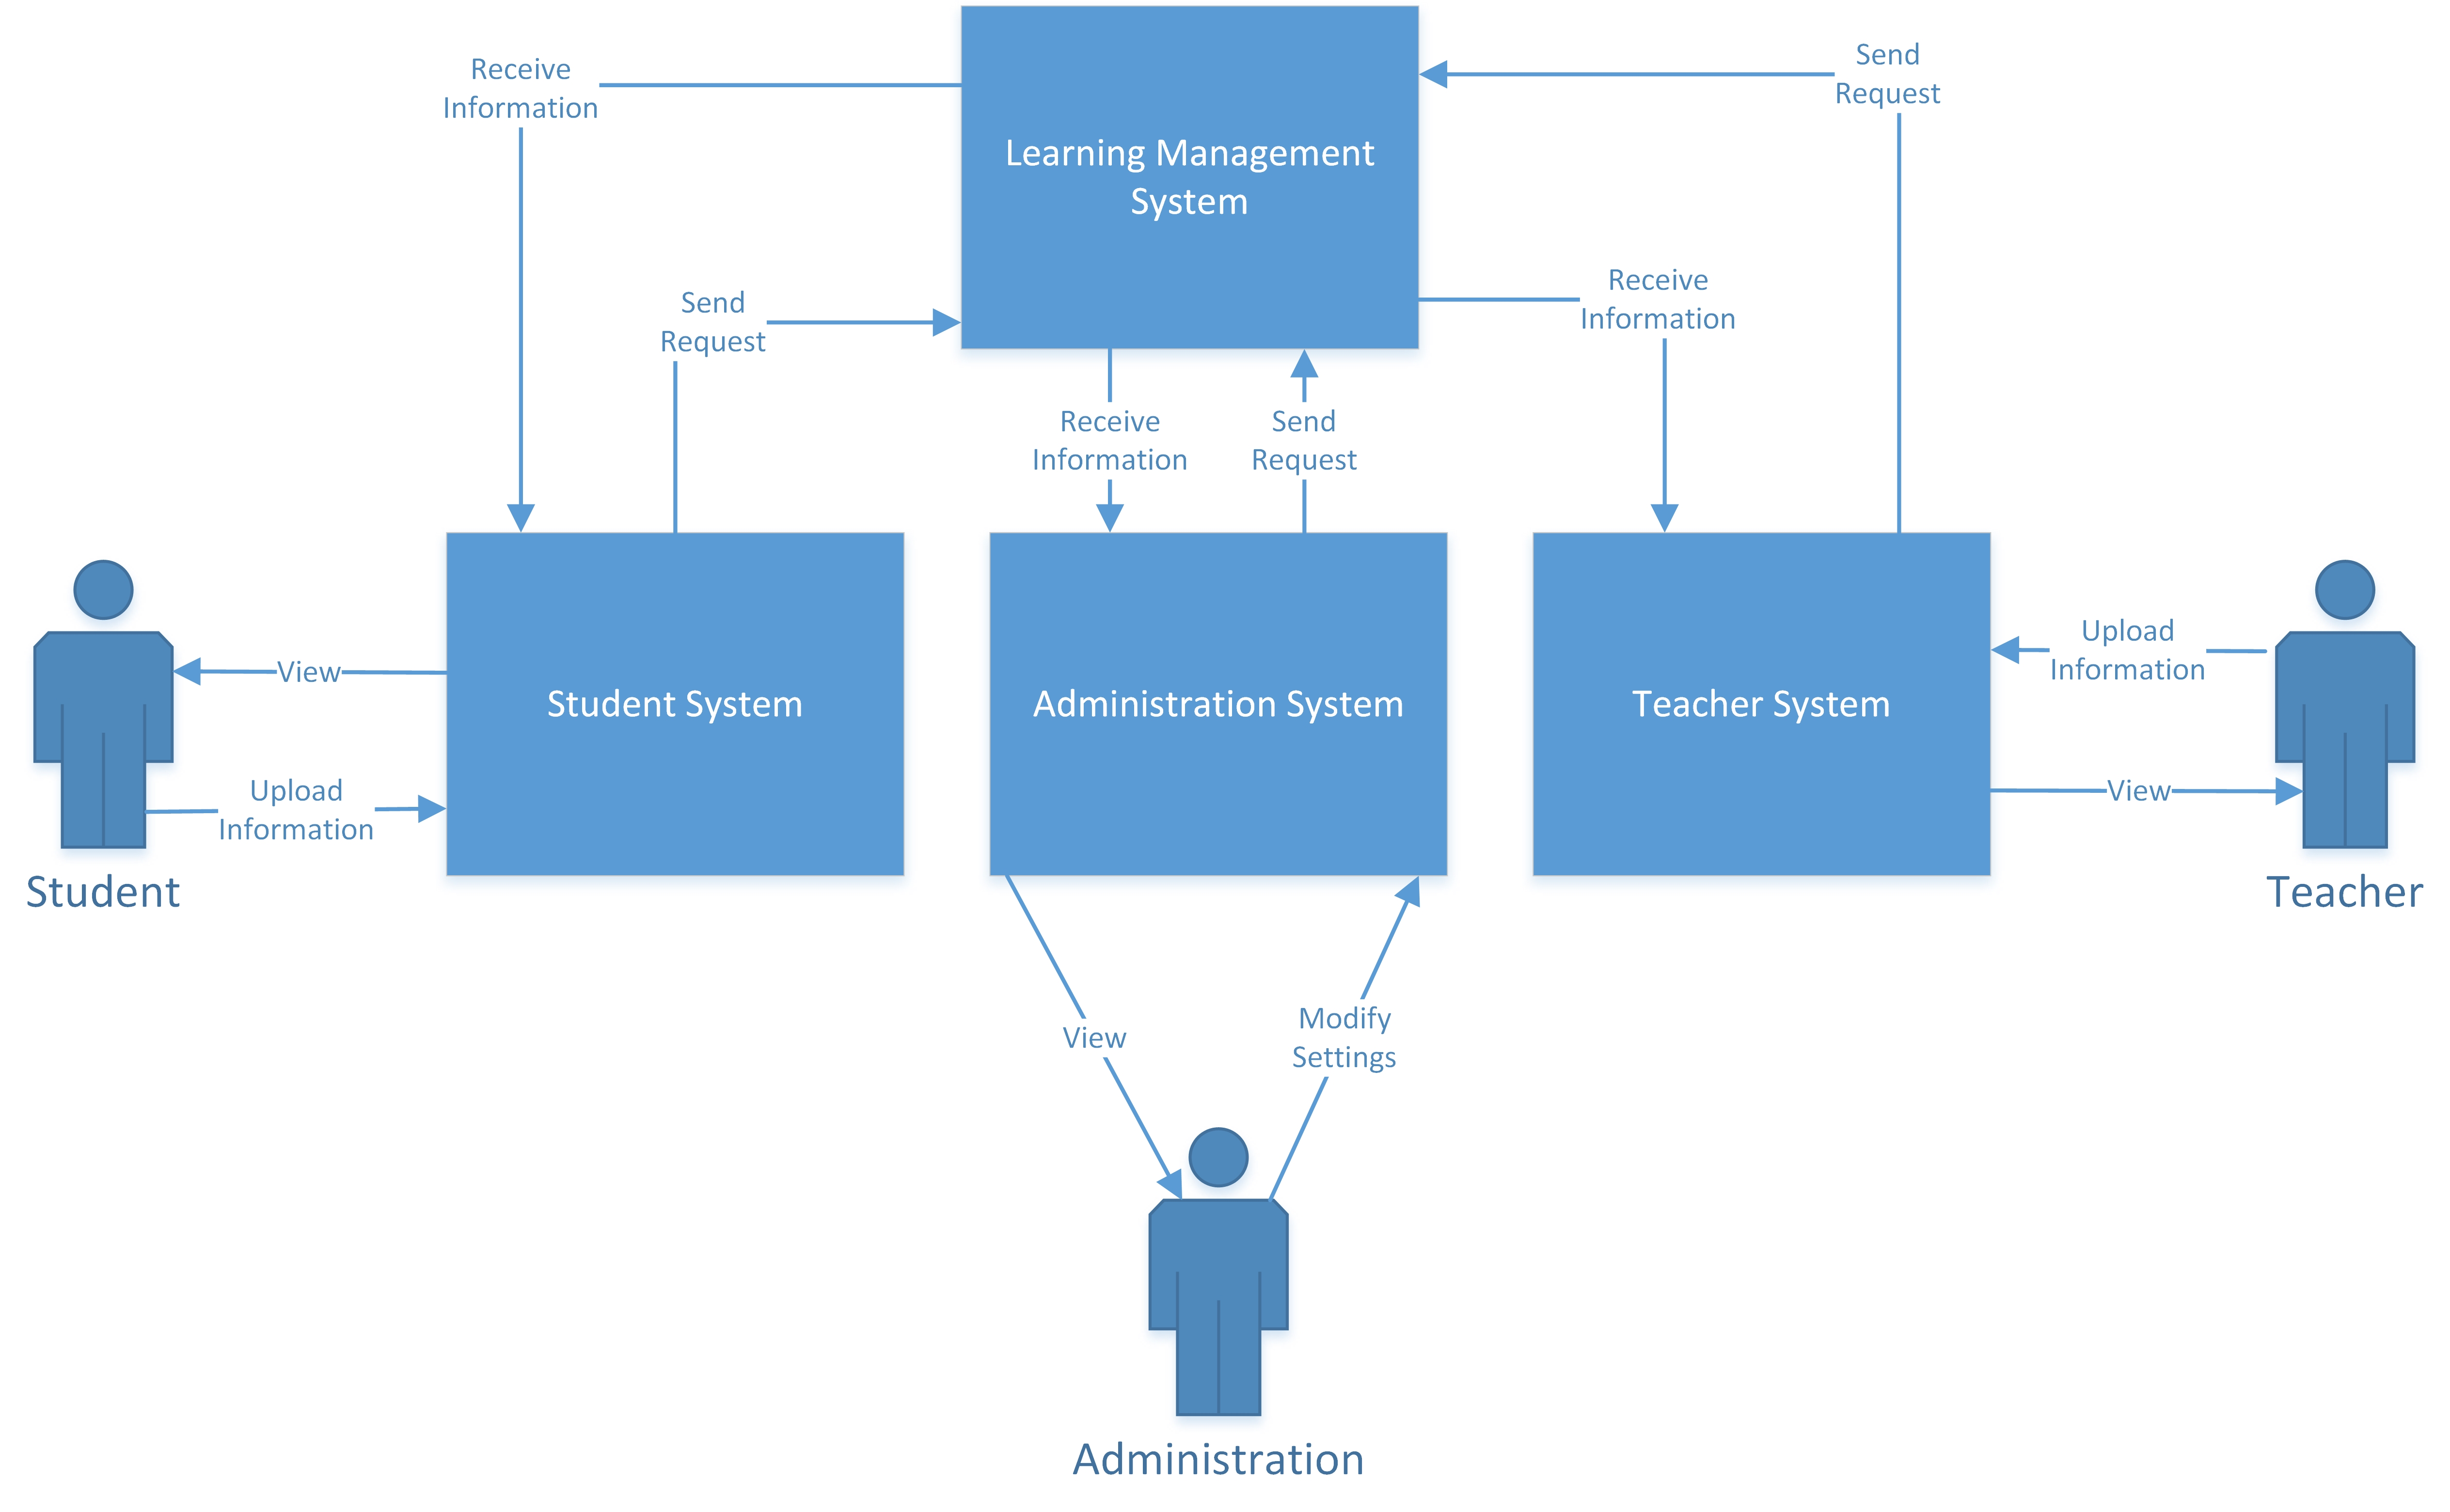
\includegraphics[scale=0.7]{A1_Assets/2-1_Product_Perspective_Diagram.jpg}
\end{center}

% End SubSection

\subsection{Product Functions}
\label{sub:product_functions}
% Begin SubSection
\begin{enumerate}[a)]
	\item Provide a summary of the major functions that the software will perform.
	\begin{itemize}
		\item \textbf{Example}: An SRS for an accounting program may use this part to address customer account maintenance, customer statement, and invoice preparation without mentioning the vast amount of detail that each of those functions requires.
	\end{itemize}
	\item Functions should be organized in a way that makes the list of functions understandable to the customer or to anyone else reading the document for the first time
	\item Textual or graphical methods can be used to show the different functions and their relationships
	\begin{itemize}
		\item Such a diagram is not intended to show a design of a product, but simply shows the logical relationships among variables
	\end{itemize}
\end{enumerate}
% End SubSection

\subsection{User Characteristics}
\label{sub:user_characteristics}
% Begin SubSection
\begin{enumerate}[a)]
	\item Describe those general characteristics of the intended users of the product including educational level, experience, and technical expertise
	\item Do not state specific requirements, but rather provide the reasons why certain specific requirements are later specified
\end{enumerate}
% End SubSection

\subsection{Constraints}
\label{sub:constraints}
% Begin SubSection
\begin{enumerate}[a)]
	\item Provide a general description of any other items that will limit the developer's options
\end{enumerate}
% End SubSection

\subsection{Assumptions and Dependencies}
\label{sub:assumptions_and_dependencies}
% Begin SubSection
\begin{enumerate}[a)]
	\item List each of the factors that affect the requirements stated in the SRS
	\item These factors are not design constraints on the software but are, rather, any changes to them that can affect the requirements in the SRS
	\begin{itemize}
		\item \textbf{Example}: An assumption may be that a specific operating system will be available on the hardware designated for the software product. If, in fact, the operating system is not available, the SRS would then have to change accordingly.
	\end{itemize}
\end{enumerate}
% End SubSection

\subsection{Apportioning of Requirements}
\label{sub:apportioning_of_requirements}
% Begin SubSection
\begin{enumerate}[a)]
	\item Identify requirements that may be delayed until future versions of the system
\end{enumerate}
% End SubSection

% End Section

\section{Functional Requirements}
\label{sec:functional_requirements}
% Begin Section
This section of the SRS should contain all of the software requirements to a level of detail sufficient to enable designers to design a system to satisfy those requirements, and testers to test that the system satisfies those requirements. Throughout this section, every stated requirement should be externally perceivable by users, operators, or other external systems. These requirements should include at a minimum a description of every input (stimulus) into the system, every output (response) from the system, and all functions performed by the system in response to an input or in support of an output.

You normally have two options for organizing your functional requirements:
\begin{enumerate}
	\item Organize first by \emph{business events}, then by \emph{viewpoints}
	\item Organize first by \emph{viewpoints}, then by \emph{business events}
\end{enumerate}
Choose the one which makes the most sense.

For example, if you wish to organization by business events:

% It is assumed that we will take this approach.
%
\begin{enumerate}[{BE}1.]
	\item A teacher must be able to create a course and own it or delete an existing course the teacher owns.
	\begin{enumerate}[{VP1}.1]
		\item Student Viewpoint
			\begin{enumerate}
				\item Students must be able to enroll in a course owned by a teacher.
			\end{enumerate}
		\item Teacher Viewpoint
			\begin{enumerate}
				\item A teacher may choose to unenroll a student from a course that the teacher owns.
				\item A teacher is not enrolled in a course.
			\end{enumerate}
		\item Parent Viewpoint
			\begin{enumerate}
				\item Should a parent wish to see their course progress or student performance, they are required to use the child's student account.
			\end{enumerate}
		\item School Administration Viewpoint
			\begin{enumerate}
				\item The school administration may choose to either allow students and teachers to create their own accounts, or create accounts for all students and teachers.
			\end{enumerate}
		\item Information Technology Team Viewpoint
			\begin{enumerate}
				\item None
			\end{enumerate}
		\item Government \& School Board Viewpoint
			\begin{enumerate}
				\item All courses, course content, and any teacher student communication held on the CMS must be made visible to the School Board.
			\end{enumerate}
	\end{enumerate}

	\item A teacher must be able to add non-evaluational, manual-evaluational and automated-evaluational content to a course created by that teacher.
	\begin{enumerate}[{VP1}.1]
		\item Student Viewpoint
			\begin{enumerate}
				\item A student enrolled in a course may view any content within the course provided the content is set visible by the owner of that course.
				\item A student may submit a piece of content in response to a manual-evaluational content provided the manual-evaluational content is set visible by the owner of that course.
				\item A student may submit an automated evaluational content provided it is set visible by the owner of that course.
			\end{enumerate}
		\item Teacher Viewpoint
			\begin{enumerate}
				\item Non-evaluational content is any content for which students are given only the option to view the content.
				\item Manual-evaluational content is any content where, in addition to viewing, students may post their own content in response, called a submitted assignment, to the content posted by the teacher.
				\item Automated-evaluational content is any content that when accessed by students, allows students to interact with that content and the result of their interaction is marked by a previously defined success criteria defined by the owner of the course.
				\item The student's performance in the exploration of automated-evaluational content is recorded and saved for future reference by the student and the teacher.
			\end{enumerate}
		\item Parent Viewpoint
			\begin{enumerate}
				\item None
			\end{enumerate}
		\item School Administration Viewpoint
			\begin{enumerate}
				\item None
			\end{enumerate}
		\item Information Technology Team Viewpoint
			\begin{enumerate}
				\item None
			\end{enumerate}
		\item Government \& School Board Viewpoint
			\begin{enumerate}
				\item None
			\end{enumerate}
	\end{enumerate}

	\item A teacher must be able view a submitted assignment. Then may choose to assign either a numerical or letter grade to the assignment.
	\begin{enumerate}[{VP2}.1]
		\item Student Viewpoint
			\begin{enumerate}
				\item Students may submit assignments multiple times in response to a manual-evaluational content posted by the course owner.
			\end{enumerate}
		\item Teacher Viewpoint
			\begin{enumerate}
				\item None
			\end{enumerate}
		\item Parent Viewpoint
			\begin{enumerate}
				\item None
			\end{enumerate}
		\item School Administration Viewpoint
			\begin{enumerate}
				\item None
			\end{enumerate}
		\item Information Technology Team Viewpoint
			\begin{enumerate}
				\item None
			\end{enumerate}
		\item Government \& School Board Viewpoint
			\begin{enumerate}
				\item None
			\end{enumerate}
	\end{enumerate}

	\item A teacher must be able to add a quiz or delete an existing quiz.
	\begin{enumerate}[{VP2}.1]
		\item Student Viewpoint
			\begin{enumerate}
				\item None
			\end{enumerate}
		\item Teacher Viewpoint
			\begin{enumerate}
				\item None
			\end{enumerate}
		\item Parent Viewpoint
			\begin{enumerate}
				\item None
			\end{enumerate}
		\item School Administration Viewpoint
			\begin{enumerate}
				\item None
			\end{enumerate}
		\item Information Technology Team Viewpoint
			\begin{enumerate}
				\item None
			\end{enumerate}
		\item Government \& School Board Viewpoint
			\begin{enumerate}
				\item None
			\end{enumerate}
	\end{enumerate}

	\item The owner of a course must be able to specify a time period for which a non-evaluational, automated-evaluational, manual-evaluational or a course is visible for to all enrolled students.
	\begin{enumerate}[{VP2}.1]
		\item Student Viewpoint
			\begin{enumerate}
				\item An enrolled student may not view content which is not made visible by the owner of the course.
			\end{enumerate}
		\item Teacher Viewpoint
			\begin{enumerate}
				\item A teacher may choose to permanently remove a piece of content from a course owned by them.
			\end{enumerate}
		\item Parent Viewpoint
			\begin{enumerate}
				\item None
			\end{enumerate}
		\item School Administration Viewpoint
			\begin{enumerate}
				\item None
			\end{enumerate}
		\item Information Technology Team Viewpoint
			\begin{enumerate}
				\item None
			\end{enumerate}
		\item Government \& School Board Viewpoint
			\begin{enumerate}
				\item None
			\end{enumerate}
	\end{enumerate}

	\item A student must be able to enroll within a course that is set visible by the owner of that course.
	\begin{enumerate}[{VP2}.1]
		\item Student Viewpoint
			\begin{enumerate}
				\item A student must be able view all courses to which they are enrolled.
				\item A student may not self withdraw from a course in which he or she is enrolled.
				\item A student that is dismissed from a course is not longer enrolled in that course.
				\item A student whom is not enrolled in a course has no access to content found within that course.
			\end{enumerate}
		\item Teacher Viewpoint
			\begin{enumerate}
				\item A teacher may dismiss an enrolled student from a course owned by the teacher.
			\end{enumerate}
		\item Parent Viewpoint
			\begin{enumerate}
				\item None
			\end{enumerate}
		\item School Administration Viewpoint
			\begin{enumerate}
				\item None
			\end{enumerate}
		\item Information Technology Team Viewpoint
			\begin{enumerate}
				\item None
			\end{enumerate}
		\item Government \& School Board Viewpoint
			\begin{enumerate}
				\item None
			\end{enumerate}
	\end{enumerate}

	\item A student must be able to view all grades assigned to them for all assignments and quizzes for all courses in which the student is enrolled.
	\begin{enumerate}[{VP2}.1]
		\item Student Viewpoint
			\begin{enumerate}
				\item None
			\end{enumerate}
		\item Teacher Viewpoint
			\begin{enumerate}
				\item None
			\end{enumerate}
		\item Parent Viewpoint
			\begin{enumerate}
				\item None
			\end{enumerate}
		\item School Administration Viewpoint
			\begin{enumerate}
				\item None
			\end{enumerate}
		\item Information Technology Team Viewpoint
			\begin{enumerate}
				\item None
			\end{enumerate}
		\item Government \& School Board Viewpoint
			\begin{enumerate}
				\item None
			\end{enumerate}
	\end{enumerate}

	\item A student must be able to view all assignments within a course in which they are enrolled provided that the owner of the course has marked them visible to be all students.
	\begin{enumerate}[{VP2}.1]
		\item Student Viewpoint
			\begin{enumerate}
				\item None
			\end{enumerate}
		\item Teacher Viewpoint
			\begin{enumerate}
				\item None
			\end{enumerate}
		\item Parent Viewpoint
			\begin{enumerate}
				\item None
			\end{enumerate}
		\item School Administration Viewpoint
			\begin{enumerate}
				\item None
			\end{enumerate}
		\item Information Technology Team Viewpoint
			\begin{enumerate}
				\item None
			\end{enumerate}
		\item Government \& School Board Viewpoint
			\begin{enumerate}
				\item None
			\end{enumerate}
	\end{enumerate}

	\item A student may submit a file in response to a manual-evaluational content only if the manual evaluational content was made visible to all students and if a submission was allowed for that student.
	\begin{enumerate}[{VP2}.1]
		\item Student Viewpoint
			\begin{enumerate}
				\item None
			\end{enumerate}
		\item Teacher Viewpoint
			\begin{enumerate}
				\item None
			\end{enumerate}
		\item Parent Viewpoint
			\begin{enumerate}
				\item None
			\end{enumerate}
		\item School Administration Viewpoint
			\begin{enumerate}
				\item None
			\end{enumerate}
		\item Information Technology Team Viewpoint
			\begin{enumerate}
				\item None
			\end{enumerate}
		\item Government \& School Board Viewpoint
			\begin{enumerate}
				\item None
			\end{enumerate}
	\end{enumerate}

	\item The school administration must be able to add a Teacher or a Student account or delete an existing Teacher or Student account.
	\begin{enumerate}[{VP1}.1]
		\item Student Viewpoint
			\begin{enumerate}
				\item The student recieves a Student ID and password to access their personal student account.
				\item The system must force student and
			\end{enumerate}
		\item Teacher Viewpoint
			\begin{enumerate}
				\item The teacher recieves a Teacher ID and password to access their personal teacher account.
			\end{enumerate}
		\item Parent Viewpoint
			\begin{enumerate}
				\item Should the parent require access to their child's account, the child is expected to login through their student account to allow the parent to inspect course progress or student performance.
			\end{enumerate}
		\item School Administration Viewpoint
			\begin{enumerate}
				\item The School Administration must be able to create batch set of user names and passwords from a CSV file.
				\item The passwords for the students and teachers are generated as follows DDMMYYYY where DDMMYYYY refers to the date of birth of the student or teacher.
			\end{enumerate}
		\item Information Technology Team Viewpoint
			\begin{enumerate}
				\item None
			\end{enumerate}
		\item Government \& School Board Viewpoint
			\begin{enumerate}
				\item It is expected that the responsibilities of monitoring communication is forwarded to the school administration. All enquiries are assumed to be forwarded to the school administration that are expected to use special access privileges to investigate issues regarding content or communication.
				\item Should any content maliagn against board policies, the school administration are given access and privileges to hide, remove or track the origin of a piece of content or course.
			\end{enumerate}
	\end{enumerate}

	\item The school administration must be able to view a course created by a Teacher or delete an existing course created by a Teacher.
	\begin{enumerate}[{VP1}.1]
		\item Student Viewpoint
			\begin{enumerate}
				\item If a course is deleted by the administration, all student data associated with that course is also deleted.
			\end{enumerate}
		\item Teacher Viewpoint
			\begin{enumerate}
				\item If a course is deleted by the administration, all teacher data associated with that course is also deleted.
			\end{enumerate}
		\item Parent Viewpoint
			\begin{enumerate}
				\item None
			\end{enumerate}
		\item School Administration Viewpoint
			\begin{enumerate}
				\item The school administration account is given a warning after a course deletion request is made. The course is deleted if and only if a course deletion request is made a second time following the warning.
			\end{enumerate}
		\item Information Technology Team Viewpoint
			\begin{enumerate}
				\item None
			\end{enumerate}
		\item Government \& School Board Viewpoint
			\begin{enumerate}
				\item It is assumed that the school administration will consult policies and procedures regarding the handling of student data.
			\end{enumerate}
	\end{enumerate}

	\item The school administration must be able to view all communication that occurs within the system between student and teachers, between student and school administration or between school administration and teachers.
	\begin{enumerate}[{VP1}.1]
		\item Student Viewpoint
			\begin{enumerate}
				\item All uploaded content or other forms of communication the student produces must be visible to all school administration accounts.
			\end{enumerate}
		\item Teacher Viewpoint
			\begin{enumerate}
				\item All uploaded content or other forms of communication the teacher produces must be visible to all school administration accounts.
			\end{enumerate}
		\item Parent Viewpoint
			\begin{enumerate}
				\item None
			\end{enumerate}
		\item School Administration Viewpoint
			\begin{enumerate}
				\item None
			\end{enumerate}
		\item Information Technology Team Viewpoint
			\begin{enumerate}
				\item None
			\end{enumerate}
		\item Government \& School Board Viewpoint
			\begin{enumerate}
				\item None
			\end{enumerate}
	\end{enumerate}

	\item Description of Business Event
	\begin{enumerate}[{VP1}.1]
		\item Student Viewpoint
			\begin{enumerate}
				\item None
			\end{enumerate}
		\item Teacher Viewpoint
			\begin{enumerate}
				\item None
			\end{enumerate}
		\item Parent Viewpoint
			\begin{enumerate}
				\item None
			\end{enumerate}
		\item School Administration Viewpoint
			\begin{enumerate}
				\item None
			\end{enumerate}
		\item Information Technology Team Viewpoint
			\begin{enumerate}
				\item None
			\end{enumerate}
		\item Government \& School Board Viewpoint
			\begin{enumerate}
				\item None
			\end{enumerate}
	\end{enumerate}

\end{enumerate}

% End Section

\section{Non-Functional Requirements}
\label{sec:non-functional_requirements}
% Begin Section
\subsection{Look and Feel Requirements}
\label{sub:look_and_feel_requirements}
% Begin SubSection

\subsubsection{Appearance Requirements}
\label{ssub:appearance_requirements}
% Begin SubSubSection
\begin{enumerate}[{LF}1. ]
	\item The application shall look aesthetically pleasing
	\item The application shall be simplistic enough for anyone to be able to use
	\item The application shall use standard fonts
	\item The application shall not have clashing colour that would make readability hard for the user
	\item The application shall look professional
	\item The application shall highlight important areas
	\item The application shall grey out choices that the user cannot make
	\item The application shall have intuitive icons as well as appropriate names to describe the function of the button
\end{enumerate}
% End SubSubSection

\subsubsection{Style Requirements}
\label{ssub:style_requirements}
% Begin SubSubSection
\begin{enumerate}[{LF}1. ]
	\item The application shall have an appropriate style for use in the classroom/professional environments
	\item The application shall be appropriate in a professional setting for teachers
	\item The application shall appeal to children
\end{enumerate}
% End SubSubSection

% End SubSection

\subsection{Usability and Humanity Requirements}
\label{sub:usability_and_humanity_requirements}
% Begin SubSection

\subsubsection{Ease of Use Requirements}
\label{ssub:ease_of_use_requirements}
% Begin SubSubSection
\begin{enumerate}[{UH}1. ]
	\item The application shall make the important features stand out and easily accessible
	\item The application shall allow the user to get to the important information with no more than 2 taps of the screen
	\item The application shall have the main feautures on the main screen where it is easy to access
	\item returning to the main screen shal
\end{enumerate}
% End SubSubSection

\subsubsection{Personalization and Internationalization Requirements}
\label{ssub:personalization_and_internationalization_requirements}
% Begin SubSubSection
\begin{enumerate}[{UH}1. ]
	\item The application shall allow the user to change the language of the application to their native language.
	\item The application shall allow the user to adjust what they want to see on the front page of the application.
	\item The application shall allow the user to adjust the order of their class
	\item The application shall allow the user to personalize their home page on the app
	\item The application shall allow the admin to change the theme of the application to appeal to teachers or students
	\item The application shall allow the user to change the language 
\end{enumerate}
% End SubSubSection

\subsubsection{Learning Requirements}
\label{ssub:learning_requirements}
% Begin SubSubSection
\begin{enumerate}[{UH}1. ]
		\item The application shall have a tutorial to outline all of the features that it has to offer the user
\end{enumerate}
% End SubSubSection

\subsubsection{Understandability and Politeness Requirements}
\label{ssub:understandability_and_politeness_requirements}
% Begin SubSubSection
\begin{enumerate}[{UH}1. ]
	\item
\end{enumerate}
% End SubSubSection

\subsubsection{Accessibility Requirements}
\label{ssub:accessibility_requirements}
% Begin SubSubSection
\begin{enumerate}[{UH}1. ]
	\item
\end{enumerate}
% End SubSubSection

% End SubSection

\subsection{Performance Requirements}
\label{sub:performance_requirements}
% Begin SubSection

\subsubsection{Speed and Latency Requirements}
\label{ssub:speed_and_latency_requirements}
% Begin SubSubSection
\begin{enumerate}[{PR}1. ]
	\item The application shall take less than 2 seconds to start up.
	\item Moving in between different parts of the application shall take less than 1 second.
\end{enumerate}
% End SubSubSection

\subsubsection{Safety-Critical Requirements}
\label{ssub:safety_critical_requirements}
% Begin SubSubSection
\begin{enumerate}[{PR}1. ]
	\item
\end{enumerate}
% End SubSubSection

\subsubsection{Precision or Accuracy Requirements}
\label{ssub:precision_or_accuracy_requirements}
% Begin SubSubSection
\begin{enumerate}[{PR}1. ]
	\item
\end{enumerate}
% End SubSubSection

\subsubsection{Reliability and Availability Requirements}
\label{ssub:reliability_and_availability_requirements}
% Begin SubSubSection
\begin{enumerate}[{PR}1. ]
	\item
\end{enumerate}
% End SubSubSection

\subsubsection{Robustness or Fault-Tolerance Requirements}
\label{ssub:robustness_or_fault_tolerance_requirements}
% Begin SubSubSection
\begin{enumerate}[{PR}1. ]
	\item
\end{enumerate}
% End SubSubSection

\subsubsection{Capacity Requirements}
\label{ssub:capacity_requirements}
% Begin SubSubSection
\begin{enumerate}[{PR}1. ]
	\item The application shall only allow 1 user/account at a time.
\end{enumerate}
% End SubSubSection

\subsubsection{Scalability or Extensibility Requirements}
\label{ssub:scalability_or_extensibility_requirements}
% Begin SubSubSection
\begin{enumerate}[{PR}1. ]
	\item
\end{enumerate}
% End SubSubSection

\subsubsection{Longevity Requirements}
\label{ssub:longevity_requirements}
% Begin SubSubSection
\begin{enumerate}[{PR}1. ]
	\item The application shall be supported and updated regularly to fix bugs and add new features
\end{enumerate}
% End SubSubSection

% End SubSection

\subsection{Operational and Environmental Requirements}
\label{sub:operational_and_environmental_requirements}
% Begin SubSection

\subsubsection{Expected Physical Environment}
\label{ssub:expected_physical_environment}
% Begin SubSubSection
\begin{enumerate}[{OE}1. ]
	\item
\end{enumerate}
% End SubSubSection

\subsubsection{Requirements for Interfacing with Adjacent Systems}
\label{ssub:requirements_for_interfacing_with_adjacent_systems}
% Begin SubSubSection
\begin{enumerate}[{OE}1. ]
	\item
\end{enumerate}
% End SubSubSection

\subsubsection{Productization Requirements}
\label{ssub:productization_requirements}
% Begin SubSubSection
\begin{enumerate}[{OE}1. ]
	\item
\end{enumerate}
% End SubSubSection

\subsubsection{Release Requirements}
\label{ssub:release_requirements}
% Begin SubSubSection
\begin{enumerate}[{OE}1. ]
	\item
\end{enumerate}
% End SubSubSection

% End SubSection

\subsection{Maintainability and Support Requirements}
\label{sub:maintainability_and_support_requirements}
% Begin SubSection

\subsubsection{Maintenance Requirements}
\label{ssub:maintenance_requirements}
% Begin SubSubSection
\begin{enumerate}[{MS}1. ]
	\item
\end{enumerate}
% End SubSubSection

\subsubsection{Supportability Requirements}
\label{ssub:supportability_requirements}
% Begin SubSubSection
\begin{enumerate}[{MS}1. ]
	\item
\end{enumerate}
% End SubSubSection

\subsubsection{Adaptability Requirements}
\label{ssub:adaptability_requirements}
% Begin SubSubSection
\begin{enumerate}[{MS}1. ]
	\item
\end{enumerate}
% End SubSubSection

% End SubSection

\subsection{Security Requirements}
\label{sub:security_requirements}
% Begin SubSection

\subsubsection{Access Requirements}
\label{ssub:access_requirements}
% Begin SubSubSection
\begin{enumerate}[{SR}1. ]
	\item
\end{enumerate}
% End SubSubSection

\subsubsection{Integrity Requirements}
\label{ssub:integrity_requirements}
% Begin SubSubSection
\begin{enumerate}[{SR}1. ]
	\item
\end{enumerate}
% End SubSubSection

\subsubsection{Privacy Requirements}
\label{ssub:privacy_requirements}
% Begin SubSubSection
\begin{enumerate}[{SR}1. ]
	\item
\end{enumerate}
% End SubSubSection

\subsubsection{Audit Requirements}
\label{ssub:audit_requirements}
% Begin SubSubSection
\begin{enumerate}[{SR}1. ]
	\item
\end{enumerate}
% End SubSubSection

\subsubsection{Immunity Requirements}
\label{ssub:immunity_requirements}
% Begin SubSubSection
\begin{enumerate}[{SR}1. ]
	\item
\end{enumerate}
% End SubSubSection

% End SubSection

\subsection{Cultural and Political Requirements}
\label{sub:cultural_and_political_requirements}
% Begin SubSection

\subsubsection{Cultural Requirements}
\label{ssub:cultural_requirements}
% Begin SubSubSection
\begin{enumerate}[{CP}1. ]
	\item
\end{enumerate}
% End SubSubSection

\subsubsection{Political Requirements}
\label{ssub:political_requirements}
% Begin SubSubSection
\begin{enumerate}[{CP}1. ]
	\item
\end{enumerate}
% End SubSubSection

% End SubSection

\subsection{Legal Requirements}
\label{sub:legal_requirements}
% Begin SubSection

\subsubsection{Compliance Requirements}
\label{ssub:compliance_requirements}
% Begin SubSubSection
\begin{enumerate}[{LR}1. ]
	\item
\end{enumerate}
% End SubSubSection

\subsubsection{Standards Requirements}
\label{ssub:standards_requirements}
% Begin SubSubSection
\begin{enumerate}[{LR}1. ]
	\item
\end{enumerate}
% End SubSubSection

% End SubSection

% End Section

\appendix
\section{Division of Labour}
\label{sec:division_of_labour}
% Begin Section
Include a Division of Labour sheet which indicates the contributions of each team member. This sheet must be signed by all team members.
% End Section

\newpage
\section*{IMPORTANT NOTES}
\begin{itemize}
	\item Be sure to include all sections of the template in your document regardless whether you have something to write for each or not
	\begin{itemize}
		\item If you do not have anything to write in a section, indicate this by the \emph{N/A}, \emph{void}, \emph{none}, etc.
	\end{itemize}
	\item Uniquely number each of your requirements for easy identification and cross-referencing
	\item Highlight terms that are defined in Section~1.3 (\textbf{Definitions, Acronyms, and Abbreviations}) with \textbf{bold}, \emph{italic} or \underline{underline}
	\item For Deliverable 1, please highlight, in some fashion, all (you may have more than one) creative and innovative features. Your creative and innovative features will generally be described in Section~2.2 (\textbf{Product Functions}), but it will depend on the type of creative or innovative features you are including.
\end{itemize}


\end{document}
%------------------------------------------------------------------------------
